\subsection{Data Analysis and Evaluation}
After the ray-tracing simulation completes, the data generated is analysed to evaluate the performance of the sensor topology. 

This component evaluates the performance of the system at each step along the trajectory of the source plane. The analysis uses data stored in the $results-\\.csv$ and $sensor\_results.csv$ output files to calculate and visualise hit efficiency. 

\subsubsection{Result Analysis Function: \texttt{plot\_hit\_percentage()}}

This script evaluates the system’s ray interception efficiency across the arc rotation of the source plane, generating two plots:

\paragraph{\textbf{Overall Hit Percentage per Arc Index}}

This plot displays the proportion of emitted rays that successfully reach any of the defined sensor areas for each simulation index (arc position). The hit percentage is calculated as:
\begin{equation}
    \text{Hit (\%)} = \frac{\text{Number of Hits}}{\text{Total Number of Rays}} \times 100
    \label{eq:Overall_Hit_Percentage}
    \addequation{Overall Hit Results (\%)}
    \end{equation}

\paragraph{\textbf{Per-Sensor Hit Percentage}}
Gaining spatial resolution of the intersection behaviours, the second subplot shows the relative 'illumination' of each sensor based on the total hits. For every arc index, the number of rays detected by each sensor is normalised by the total number of hits. This allows identification of the directional coverage for each sensor. 

\begin{figure}[htbp] %h-ere t-op b-ottom p-page (separte) -good to allow all htbp to give the compiler more options
    \centering
    \includegraphics[width=0.8\textwidth]{chapters/methodology/SoftwareModel/images/plot\_hit\_percentage\_combined.png} % change {path}
    \caption{\texttt{plot\_hit\_percentage()} Output Plot}       % change {caption}
    \label{fig:Hit Percentage Output Plot}            % change label - used for reference in text
\end{figure}                             % for example: see in Figure~\ref{example label}

\vspace{1em}
Together these visualisations form an overview of the sensor system's performance and directional sensitivity. 

\subsubsection{Sensor Spatial Response Function: \texttt{sensor\_surface\_plots()}}
While previous analysis plots visualise results per arc index, this function presents a higher-dimensional insight by mapping each sensor’s illumination response across both the arc angle and the tilt angle. The underlying data is drawn from \texttt{sensor\_results.csv} and the angular mapping in \texttt{rigid\_arc\_angles.csv}.

Each output is a 3D surface plot, Figure~\ref{fig:Sensor Surface Output Plot}, where:
\begin{itemize}
    \item The $x$-axis represents the \textbf{arc angle} (horizontal angular sweep),
    \item The $y$-axis represents the \textbf{tilt angle} (vertical angular sweep),
    \item The $z$-axis shows the \textbf{number of ray hits} for each sensor.
\end{itemize}
This visualisation allows for an evaluation of the angular coverage of each sensor and the orthogonality of the measurements.
\begin{landscape}
    \begin{figure}[p] %h-ere t-op b-ottom p-page (separte) -good to allow all htbp to give the compiler more options
        \centering
        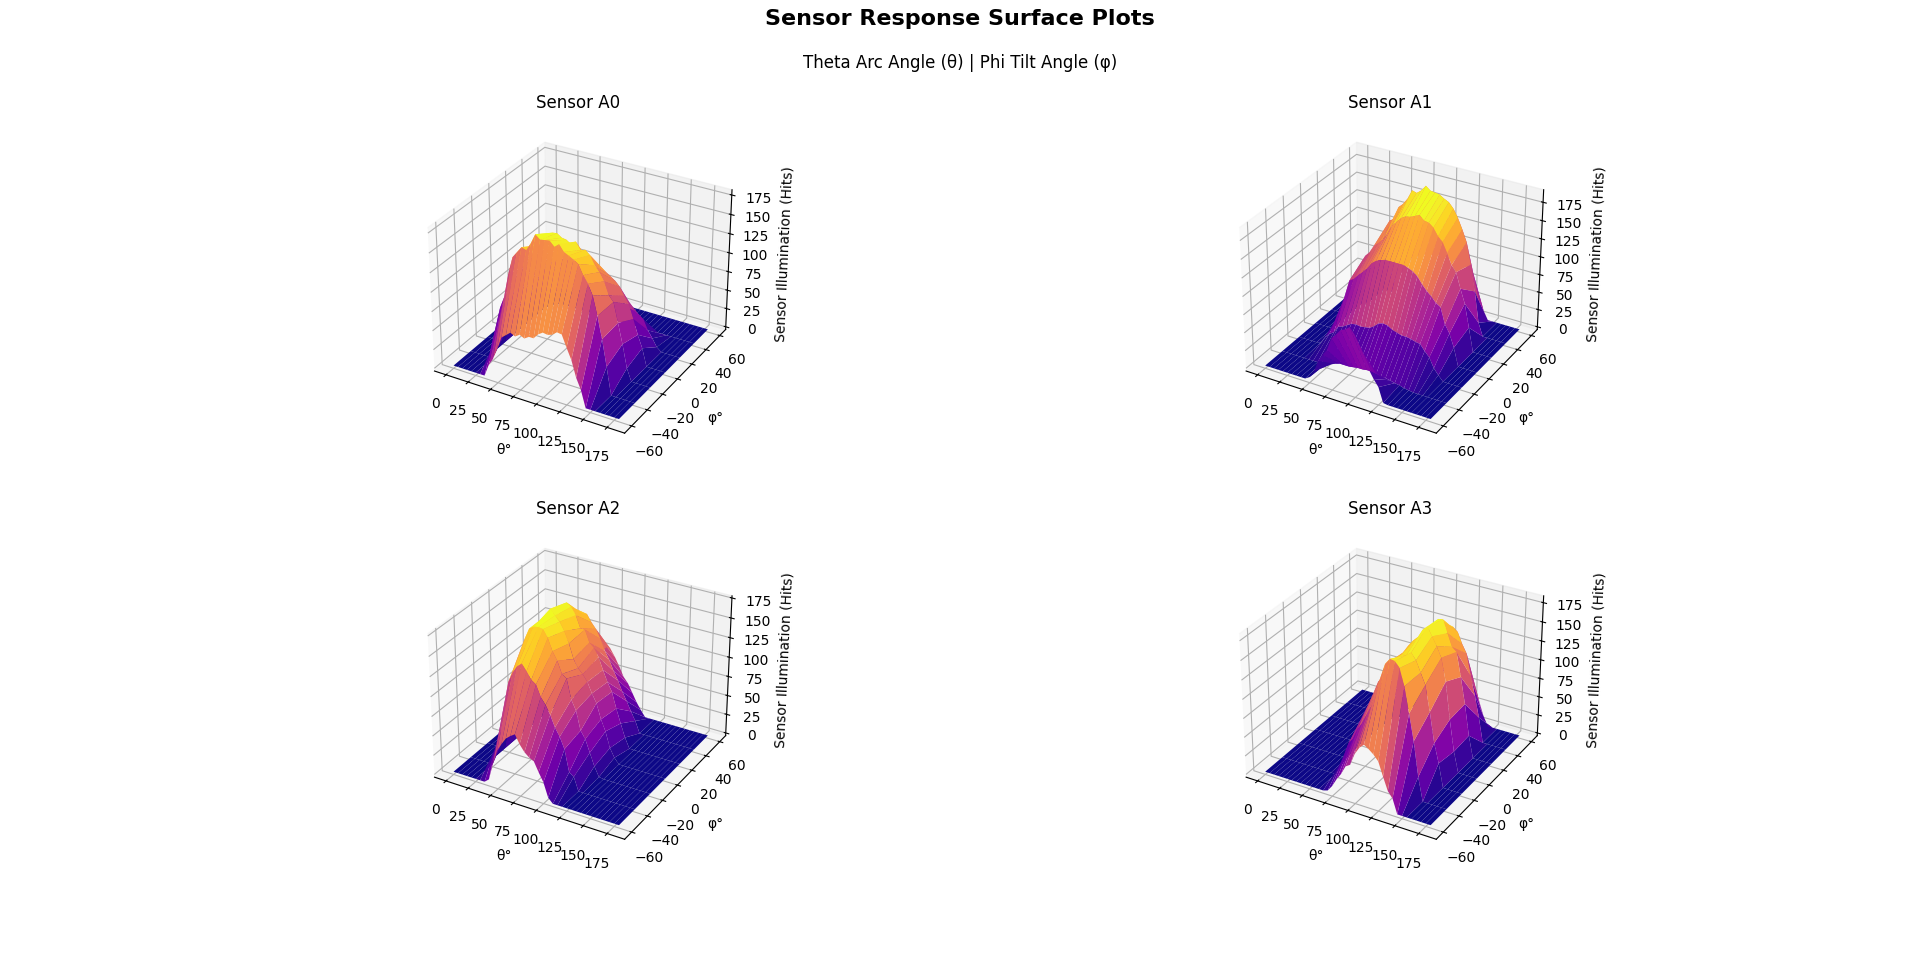
\includegraphics[width=1\textwidth]{chapters/methodology/SoftwareModel/images/Sensor Surface Plots.png} % change {path}
        \caption{\texttt{sensor\_surface\_plots()} Output Plot}       % change {caption}
        \label{fig:Sensor Surface Output Plot}            % change label - used for reference in text
    \end{figure}
\end{landscape}

\subsubsection{Model Testing}
To validate the functionality of the model test configurations were created. Each test scenario targets a specific feature or behaviour of the ray-plane interaction system, ensuring that the model behaves as expected.

The simulation framework was tested using several `.json` configuration files, each defining different spatial setups for the source, aperture, and sensor planes. The expected outcome of each test was determined analytically based on geometric relationships. Below is a summary of each test and its intended validation purpose:

\begin{itemize}
    \item \textbf{test\_arc\_rotation.json} \\
    This test evaluates the full arc movement of the source plane in a rigid semi-circular path, with multiple sensors and two distinct apertures. The simulation checks whether rays, emitted from various arc positions, are correctly filtered through the apertures and accurately detected by the sensors. \textit{Expected result:} a non-uniform distribution of sensor hits across arc positions, demonstrating correct handling of dynamic source movement and occlusion logic.
    
    \item \textbf{test\_directly\_below.json} \\
    A basic validation scenario where a single sensor is placed directly beneath a uniformly open aperture and source. The system is expected to demonstrate maximal efficiency under ideal alignment conditions. \textit{Expected result:} High \% ray intersection success with the sensor area.

    \item \textbf{test\_no\_intersection.json} \\
    This test ensures that rays that are directed orthogonally to the sensor plane (i.e., no downward component). The source emits horizontally, and the sensor is placed far from the expected ray path. \textit{Expected result:} zero valid intersections, confirming non-intersection conditions.

    \item \textbf{test\_off\_center.json} \\
    In this configuration, sensors are slightly offset from the central axis of the source, with a wide aperture. This test is used to assess the spatial precision of the system when determining ray hits that fall near sensor boundaries. \textit{Expected result:} a partial detection pattern, with hits concentrated on central sensors and misses on outer ones depending on angular spread.

    \item \textbf{test\_with\_aperture.json} \\
    This test includes two apertures spatially separated along the y-axis and a single sensor aligned with one of them. It is intended to verify whether rays are correctly filtered by the aperture before reaching the sensor. \textit{Expected result:} Most rays intersect outside aligned apertures, with sensor registering hits only through valid aperture intersecting paths.

\end{itemize}

Together, these tests provide functional validation of the core components: ray generation, source arc trajectory, aperture filtering, and intersection logic. The system’s ability to handle edge cases (e.g., no intersection, misalignment) supports its robustness and practical viability for analysis and experimentation of potential sensor topologies.

\subsubsection{Model Evaluation Function: \texttt{Run Time and Hit Gain Efficiency}}

The second aspect focuses on the computational performance of the simulation in relation to the effects of increasing the number of rays.
This is implemented in the $plot\_runtime\_vs\_gain()$ function, which processes $results.csv$ to compute:

\paragraph{\textbf{Average Runtime per Ray Count}}

- The mean execution time required for the simulation of varying ray counts, providing a baseline for understanding the simulation's computational demands.

\paragraph{\textbf{Marginal Gain in Hit Percentage}}
- This quantifies how much additional hit accuracy is gained by increasing the number of rays. It is computed by taking the difference in hit percentage between successive ray counts. This helps to identify the point(s) of diminishing returns, where increasing the ray count leds to diminishing returns in terms of accuracy.

\paragraph{\textbf{Cost per Percentage Gain}}
- Further quantifying efficiency, this analysis calculates the cost per 1\% gain in hit percentage. This expresses how many seconds of simulation time are required to improve accuracy by one percentage point, it provides insight into whether it is computationally justified to increase ray count. 

\begin{equation}
    \text{Cost per Gain} = \frac{\Delta \text{Runtime}}{\Delta \text{Hit Percentage}}
    \label{eq:Cost_per_Gain}
    \addequation{Cost per Gain accuracy}
\end{equation}

\vspace{1em}


\begin{figure}[htbp] %h-ere t-op b-ottom p-page (separte) -good to allow all htbp to give the compiler more options
    \centering
    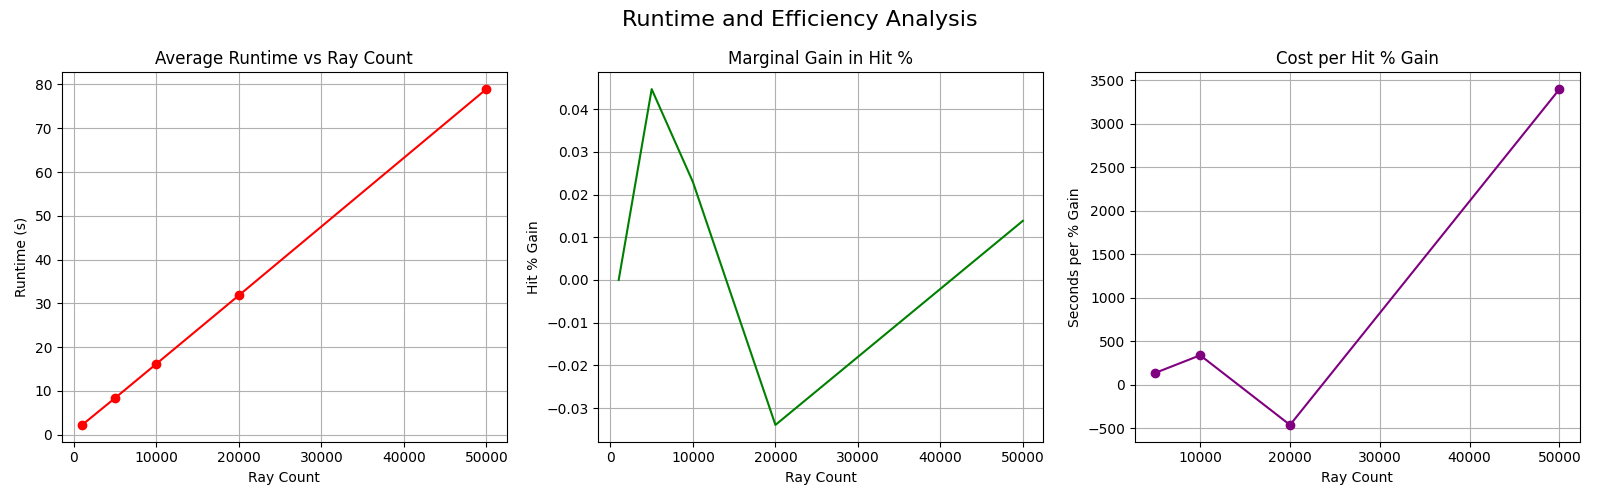
\includegraphics[width=0.9\textwidth]{chapters/methodology/SoftwareModel/images/run time analysis.png} % change {path}
    \caption{\texttt{Run Time and Hit Gain Efficiency} Output Plot}       % change {caption}
    \label{fig:Run Time and Hit Gain Efficiency}            % change label - used for reference in text
\end{figure}  

These results help in determining the optimal ray count against computational expense, ensuring that the simulation remains accuracy and practical.



    \begin{table}[h]
        \centering
        \caption{Summary of Analysis Functions}
        \label{tab:analysis_summary}
        \begin{tabular}{>{\raggedright}p{4cm} >{\raggedright}p{5cm} >{\raggedright\arraybackslash}p{5cm}}
            \toprule
            \textbf{Function} & \textbf{Metrics Generated} & \textbf{Purpose} \\
            \midrule
            \texttt{plot\_hit\_percentage \_combined()} & Overall Hit Percentage \newline Per-Sensor Hit Distribution & Assess ray interception performance and directional sensitivity \\
            \texttt{plot\_runtime\_vs \_gain()} & Average Runtime \newline Marginal Gain in Hit \% \newline Cost per Gain & Evaluate efficiency vs. accuracy trade-offs in ray count configuration \\
            \texttt{sensor\_surface \_plots()} & Sensor Response 3D Surfaces & Visualise angular response behaviour of each sensor across the full tilt/arc space \\
            \bottomrule
        \end{tabular}
    \end{table}
